Оценку эффективности протоколов будем проводить по двум
параметрам:

\begin{itemize}
	\item время от начала до конца передачи в секундах – $t$;
	\item коэффициент эффективности $k$ -- количество всех пакетов, поделенных на общее количество отправлений.
\end{itemize}

Для оценки эффективности была проведена серия экспериментов с
различными значениями размера окна и вероятности потери пакетов. Во всех
тестах количество передаваемых пакетов равно 100, lost\_timeout = 0.2 с. В силу того, что оба показателя эффективности зависят от случая, то для робастности все исследования повторяются несколько раз, а значения параметров, полученные в разных повторениях и при одинаковых условиях, усредняются. 

Зависимость коэффициента эффективности $k$ и времени передачи $t$ от
вероятности потери пакета $p$ при фиксированном размере окна
window\_size = 3 представлена в таблице 1 и графически на рис. 4. В данном случае каждое значение получалось путем усреднения соответствующих параметров эффективности при 3 повторениях.

\begin{figure}[H]
	\begin{center}
		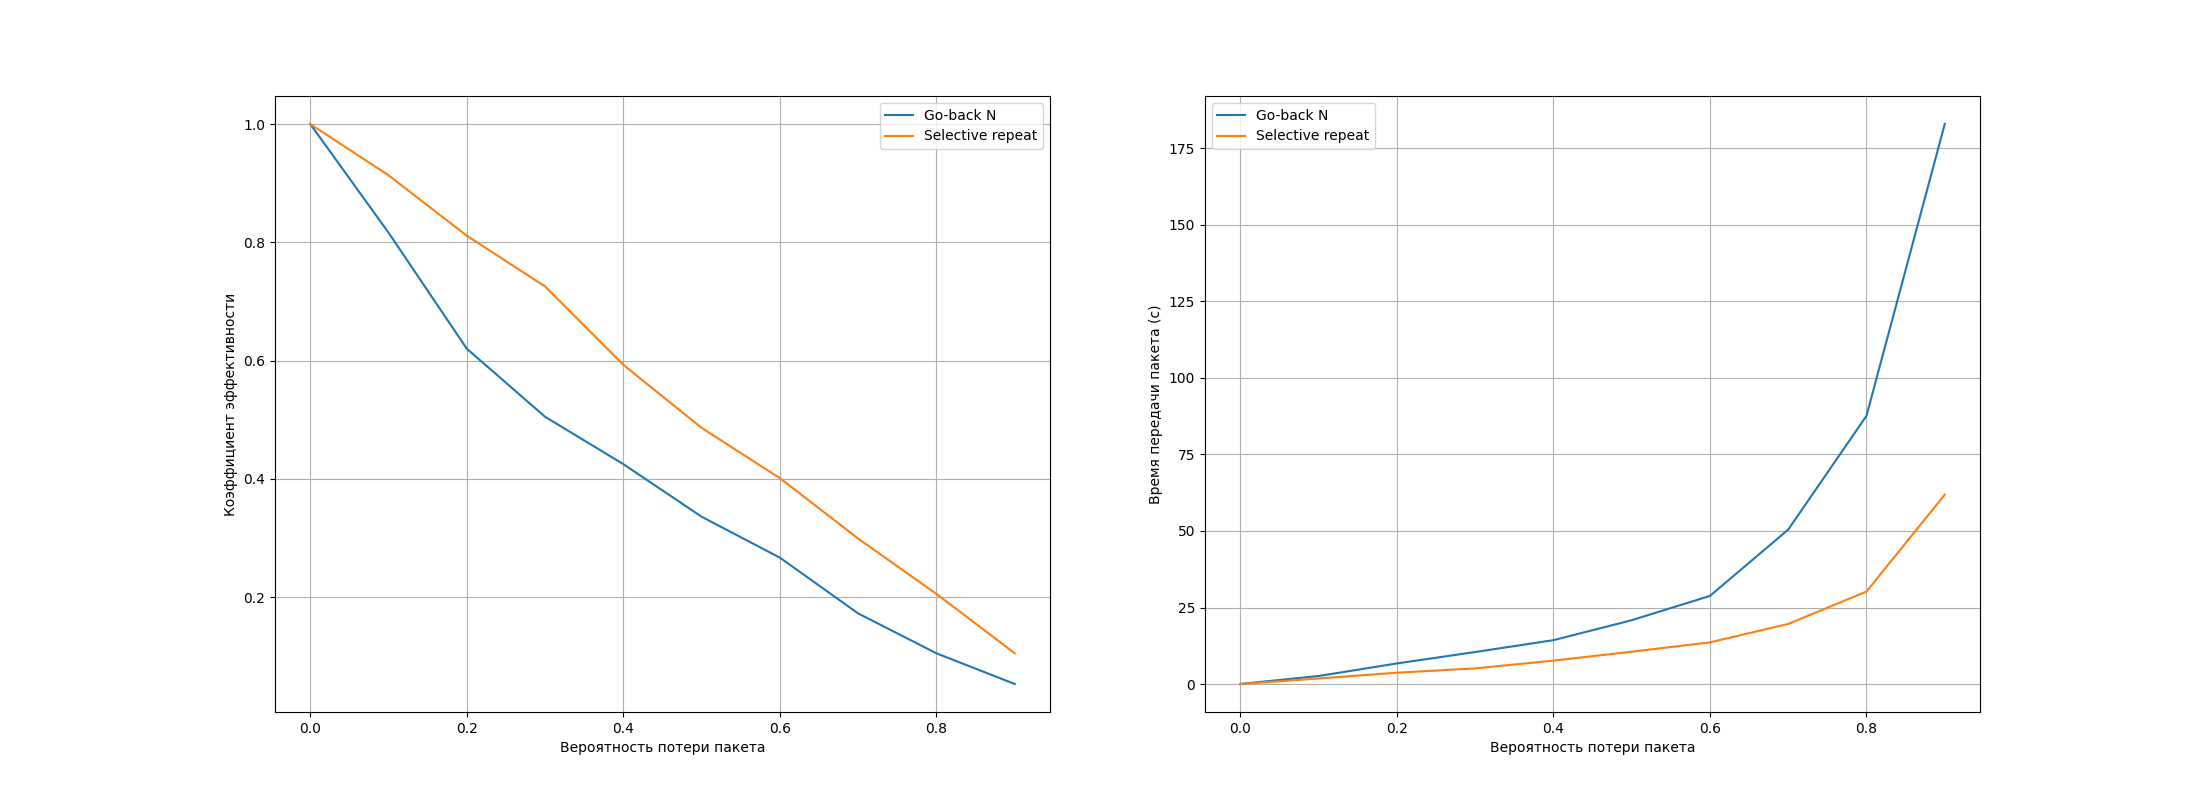
\includegraphics[scale=0.35]{prob_test.png}
		\caption{Визуализация передачи данных с использованием скользящего окна}
	\end{center}
\end{figure}

\begin{table}[H]
	\begin{center}
		\begin{tabular}{|c|c|c|c|c|}
			\hline
			 & \multicolumn{2}{c|}{Go-Back N} & \multicolumn{2}{c|}{Selective Repeat} \\
			\hline
			$p$ & $t (sec)$ & $k$ & $t (sec)$ & $k$ \\
			\hline
			0.0 & 0.04 & 1.00 & 0.03 & 1.00 \\
			\hline
			0.1 & 2.64 & 0.816 & 1.83 & 0.91\\
			\hline
			0.2 & 6.73 & 0.62 & 3.73 & 0.81\\
			\hline
			0.3 & 10.47 & 0.50 & 5.13 & 0.73\\
			\hline
            0.4 & 14.34 & 0.42 & 7.67 & 0.6\\
			\hline
			0.5 & 20.85 & 0.33 & 10.57 & 0.49\\
			\hline
			0.6 & 28.8 & 0.26 & 13.62 & 0.40\\
			\hline
			0.7 & 50.45 & 0.17 & 19.64 & 0.30\\
			\hline
			0.8 & 87.62 & 0.10 & 30.22 & 0.21\\
			\hline
			0.9 & 182.91 & 0.05 & 61.87 & 0.11\\
			\hline
		\end{tabular}
		\caption{ Зависимость показателей параметров эффективности протоколов от вероятности потери пакета при window\_size = 3}
	\end{center}
\end{table}


Зависимость
эффективности $k$ и времени передачи $t$ от размера окна window\_size при
заданной вероятности потери пакета $p = 0.3$ представлена в табл. 2 и на рис. 5. В данном случае показатели параметров эффективности были более хаотичными, потому усреднение значений производилось по 30 замерам. 

\begin{figure}[H]
	\begin{center}
		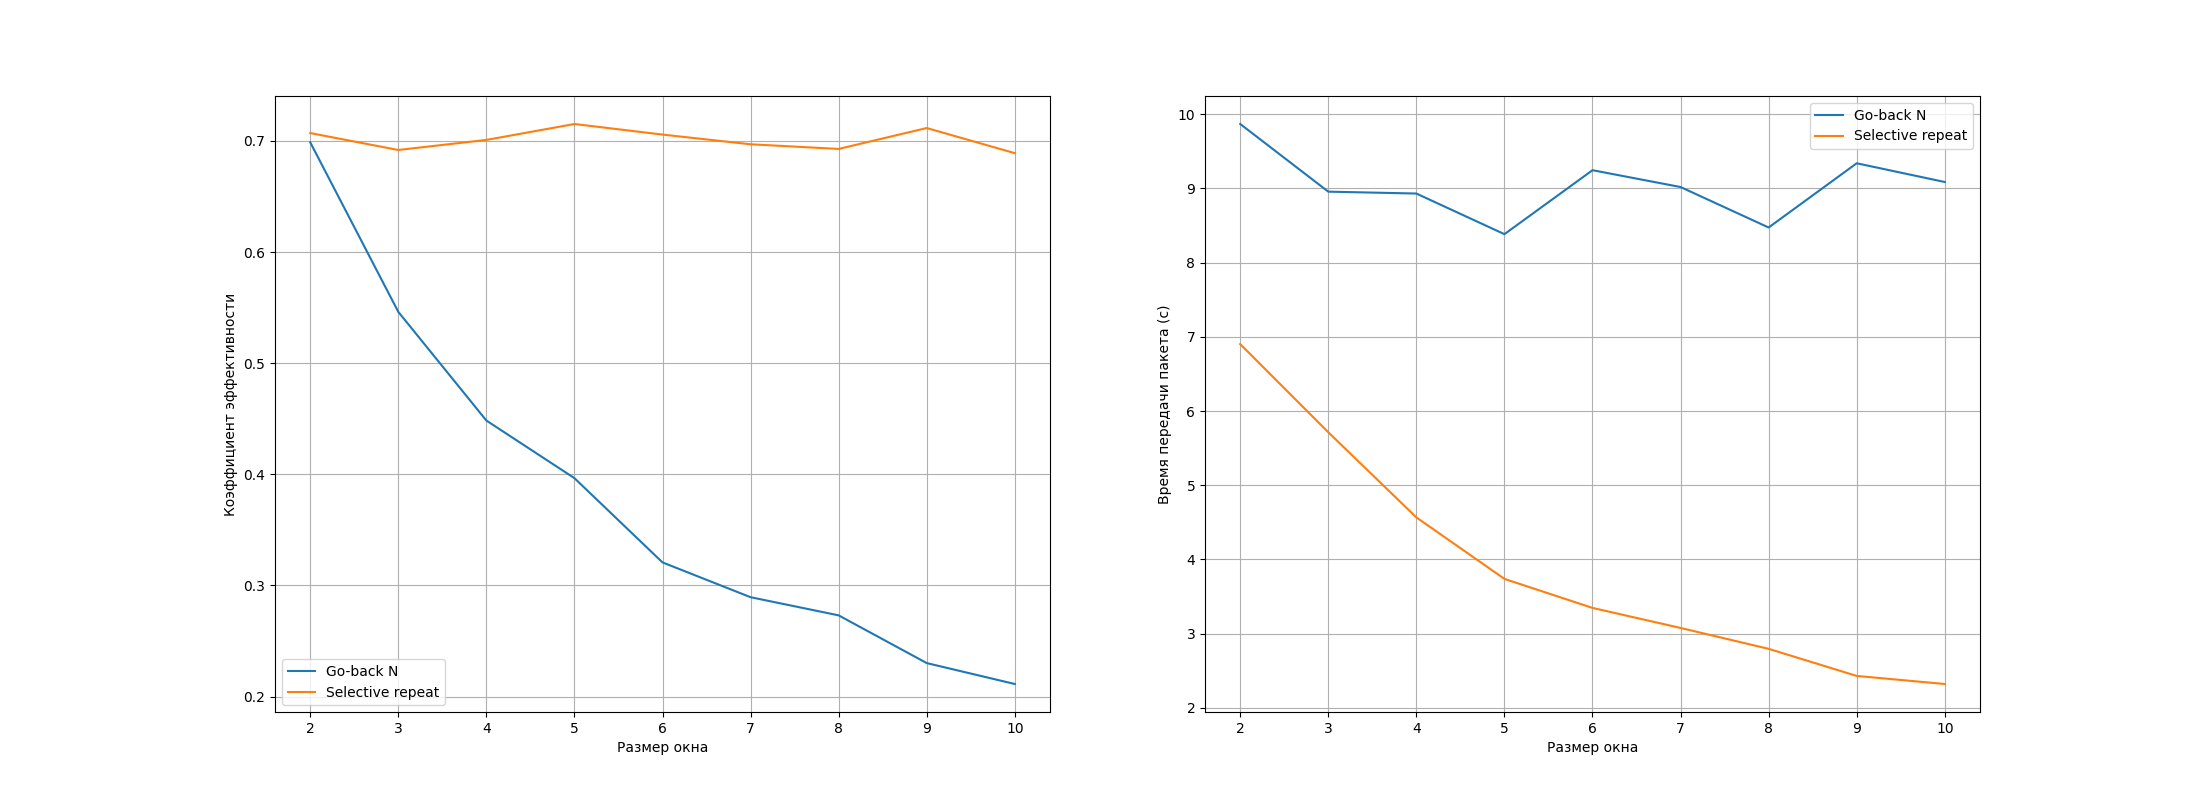
\includegraphics[scale=0.35]{ws_test.png}
		\caption{Зависимость коэффициента эффективности (слева) и времени передачи (справа) от размера окна при $p = 0.3$}
	\end{center}
\end{figure}

\begin{table}[H]
	\begin{center}
		\begin{tabular}{|c|c|c|c|c|}
			\hline
			& \multicolumn{2}{c|}{Go-BackN} & \multicolumn{2}{c|}{Selective Repeat} \\
			\hline
			window size & $t (sec)$ & $k$ & $t (sec)$ & $k$ \\
			\hline
			2 & 9.87 & 0.69 & 6.9 & 0.7 \\
			\hline
			3 & 8.95 & 0.54 & 5.7 & 0.69\\
			\hline
			4 & 8.93 & 0.44 & 4.57 & 0.7\\
			\hline
			5 & 8.38 & 0.4 & 3.74 & 0.71\\
			\hline
			6 & 9.24 & 0.32 & 3.35 & 0.71\\
			\hline
			7 & 9.02 & 0.29 & 3.1 & 0.7\\
			\hline
			8 & 8.47 & 0.27 & 2.8 & 0.7\\
			\hline
			9 & 9.34 & 0.23 & 2.43 & 0.71\\
			\hline
			10 & 9.09 & 0.21 & 2.32 & 0.69\\
			\hline
		\end{tabular}
		\caption{Зависимость показателей параметров эффективности протоколов от размера окна при loss\_probability = 0.3}
	\end{center}
\end{table}
